\documentclass[9pt,aspectratio=169]{beamer}

\usepackage[utf8]{inputenc}
\usepackage[T1]{fontenc}
\usepackage{lmodern}
\usepackage{microtype}
\usepackage[english]{babel}
\usepackage{booktabs}
\usepackage{array}
\usepackage{listings}
\usepackage{tikz}
\usetikzlibrary{positioning,arrows.meta,shapes.geometric}
\usepackage{xcolor}

\definecolor{bhblue}{RGB}{26,84,162}
\definecolor{bhgray}{RGB}{80,80,80}
\definecolor{codebg}{HTML}{F5F5F5}
\definecolor{ccwarm}{HTML}{D97757}

\usetheme{Madrid}
\usecolortheme{seahorse}
\setbeamercolor{title}{fg=bhblue}
\setbeamercolor{frametitle}{fg=bhblue}
\setbeamercolor{block title}{bg=bhblue,fg=white}
\hypersetup{colorlinks=true, linkcolor=bhblue, urlcolor=bhblue}

\setbeamertemplate{navigation symbols}{}
\setbeamertemplate{footline}{}
\setbeamersize{text margin left=0.9cm,text margin right=0.9cm}
\setlength{\parskip}{0.2em}
\setbeamerfont{frametitle}{size=\large}

\lstdefinestyle{shell}{
  basicstyle=\ttfamily\footnotesize,
  backgroundcolor=\color{codebg},
  frame=single,
  framesep=4pt,
  rulecolor=\color{lightgray},
  breaklines=true,
  showstringspaces=false
}

\title{Data search and scraping}
\author{Sankalp Sharma}
\institute{University of Southern California}
\date{Fall 2026}

\begin{document}

% ============================================================
% 1. Cheap path first
% ============================================================
\begin{frame}{Finding and collecting data}

\begin{enumerate}
  \item Be careful with government websites
  \item Don't scrape what you don't needs
  \item \textbf{ALWAYS} check robots.txt
\end{enumerate}

TODAY's example: SEC Edgar filings
\\ 
Workflow:

  \vspace{0.1cm}
  \begin{center}
    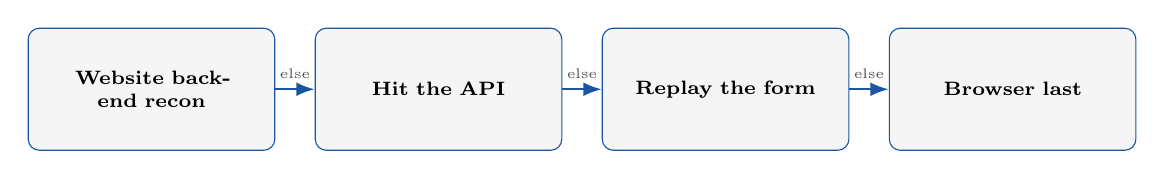
\begin{tikzpicture}[
      font=\scriptsize,
      box/.style={
        draw=bhblue, fill=codebg, rounded corners,
        align=center, text width=2.85cm, inner sep=4pt,
        minimum height=1.55cm
      },
      arr/.style={-{Latex}, thick, bhblue}
    ]
      \node[box] (file)
        {\textbf{Website backend recon}};
      \node[box, right=0.5cm of file] (api)
        {\textbf{Hit the API}};
      \node[box, right=0.5cm of api] (form)
        {\textbf{Replay the form}};
      \node[box, right=0.5cm of form] (browser)
        {\textbf{Browser last}};
      \draw[arr] (file) -- node[above, font=\tiny, text=bhgray] {else} (api);
      \draw[arr] (api) -- node[above, font=\tiny, text=bhgray] {else} (form);
      \draw[arr] (form) -- node[above, font=\tiny, text=bhgray] {else} (browser);
    \end{tikzpicture}
  \end{center}

  \vspace{0.2cm}
  Worked example: \texttt{fall-2026/sec\_edgar.py}.

\end{frame}

% ============================================================
% 2. How we wrote the script
% ============================================================
\begin{frame}{How we wrote \texttt{sec\_edgar.py}}

  We did not scrape the search page. We asked what it talks to.

  \vspace{0.12cm}
  \begin{center}
    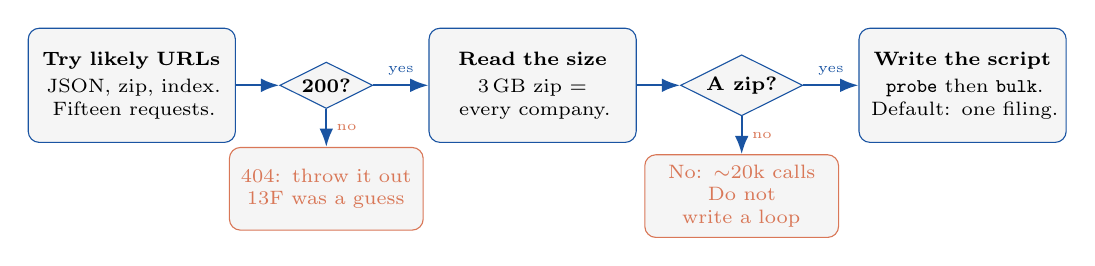
\begin{tikzpicture}[
      font=\scriptsize,
      box/.style={
        draw=bhblue, fill=codebg, rounded corners,
        align=center, text width=2.35cm, inner sep=4pt,
        minimum height=1.45cm
      },
      decision/.style={
        diamond, draw=bhblue, fill=codebg, aspect=2.0,
        align=center, inner sep=1pt, font=\scriptsize\bfseries
      },
      reject/.style={
        draw=ccwarm, fill=codebg, rounded corners,
        align=center, text width=2.25cm, inner sep=3pt,
        text=ccwarm, minimum height=1.05cm
      },
      arr/.style={-{Latex}, thick, bhblue}
    ]
      \node[box] (try)
        {\textbf{Try likely URLs}\\[2pt]
         JSON, zip, index.\\
         Fifteen requests.};
      \node[decision, right=0.55cm of try] (ok) {200?};
      \node[box, right=0.7cm of ok] (size)
        {\textbf{Read the size}\\[2pt]
         3\,GB zip $=$ every company.};
      \node[decision, right=0.55cm of size] (zip) {A zip?};
      \node[box, right=0.7cm of zip] (write)
        {\textbf{Write the script}\\[2pt]
         \texttt{probe} then \texttt{bulk}.\\
         Default: one filing.};

      \node[reject, below=0.48cm of ok] (drop)
        {404: throw it out\\13F was a guess};
      \node[reject, below=0.48cm of zip] (loop)
        {No: $\sim$20k calls\\Do not write a loop};

      \draw[arr] (try) -- (ok);
      \draw[arr] (ok) -- node[above, font=\tiny] {yes} (size);
      \draw[arr] (ok) -- node[right, font=\tiny, text=ccwarm] {no} (drop);
      \draw[arr] (size) -- (zip);
      \draw[arr] (zip) -- node[above, font=\tiny] {yes} (write);
      \draw[arr] (zip) -- node[right, font=\tiny, text=ccwarm] {no} (loop);
    \end{tikzpicture}
  \end{center}

  \vspace{0.18cm}
  \footnotesize
  Every request needs a \texttt{User-Agent} with your name and email.
  Without it you get 403, not data.

\end{frame}

% ============================================================
% 3. A new site
% ============================================================
\begin{frame}{On a new site, fingerprint the HTML first}

  Fetch the page (or have the agent fetch it) and search the source.
  The markers below pick the method.

  \vspace{0.25cm}
  \renewcommand{\arraystretch}{1.18}
  \footnotesize
  \begin{tabular}{@{}p{0.38\textwidth} p{0.54\textwidth}@{}}
    \toprule
    {\color{bhblue}\bfseries Marker} & {\color{bhblue}\bfseries First move} \\
    \midrule
    \texttt{.zip}, \texttt{.csv}, Download
      & Take the file. \\
    \texttt{/api/}, \texttt{.json}
      & Call it. Skip the HTML. \\
    \texttt{MapServer}, \texttt{FeatureServer}
      & ArcGIS. Query the layer; start with a count. \\
    \texttt{\_\_VIEWSTATE}, \texttt{.aspx}
      & WebForms. Replay the POST. Hidden tokens go stale after each click. \\
    \texttt{\_csrf}, \texttt{JSESSIONID}
      & Session token. Keep the cookie across the run. \\
    \bottomrule
  \end{tabular}

  \vspace{0.3cm}
  Then hit the candidate URLs. Record status, size, row count, whether auth is
  real, and the pagination parameter (\texttt{page}, \texttt{from}, \texttt{offset}).

  \vspace{0.12cm}
  Write \texttt{scrape/sitename\_endpoints.md}. Pick the extract after that file exists.

\end{frame}

% ============================================================
% 4. Prompt + habits
% ============================================================
\begin{frame}[fragile]{What you tell the agent}

  \vspace{0.05cm}
  \begin{columns}[T,onlytextwidth]
    \column{0.48\textwidth}
    {\footnotesize\color{ccwarm}\bfseries Skips the cheap path}
    \begin{lstlisting}[style=shell]
Scrape this website and
give me a CSV.
    \end{lstlisting}

    \column{0.48\textwidth}
    {\footnotesize\color{bhblue}\bfseries Finds it}
    \begin{lstlisting}[style=shell]
Probe candidate URLs.
Report status, size,
record count, and auth.
Write endpoints.md.
Do not write a scraper yet.
    \end{lstlisting}
  \end{columns}

  \vspace{0.22cm}
  Once the path is known, from \texttt{sec\_edgar.py}:

  \vspace{0.08cm}
  \renewcommand{\arraystretch}{1.15}
  \footnotesize
  \begin{tabular}{@{}p{0.26\textwidth} p{0.66\textwidth}@{}}
    \toprule
    {\color{bhblue}\bfseries Habit} & {\color{bhblue}\bfseries Why} \\
    \midrule
    Safe default
      & No arguments: one filing under 500\,KB. Bulk needs \texttt{--yes}. \\
    Write, then rename
      & A crash mid-write otherwise leaves a short file that resume treats as done. \\
    Test URLs offline
      & Builders and parsers have no network. \texttt{selftest} is \texttt{assert}. \\
    One bad record
      & At 20{,}000 requests some fail for reasons unrelated to your code.
        Crashing on item 4{,}000 is how you lose a night. \\
    \bottomrule
  \end{tabular}

  \vspace{0.2cm}
  \footnotesize
  Full-text search reports \texttt{\{"value": 10000, "relation": "gte"\}}.
  That is a floor. Treating it as the count drops the rest of the sample.
  The script refuses \texttt{gte} queries and tells you to slice by date.

\end{frame}

% ============================================================
% 5. Starting prompt
% ============================================================
\begin{frame}[fragile]{Starting prompt}

  Paste this first. Stop when the file exists.

\begin{lstlisting}[style=shell,columns=fullflexible]
Target: https://www.sec.gov/edgar/
Goal: find the real backend/API behind EDGAR and
document every bulk data path.
Deliverable: scrape/sec_edgar_endpoints.md -- host,
base paths, auth, record counts, pagination params,
bulk-download sizes, rate limits, with live
verification evidence.
Depth: recon only. Do not build a scraper yet.
\end{lstlisting}

\end{frame}

\end{document}
